\section{问题二：无碰撞终止时刻的判定}
\subsection{问题二的建模动机}
问题二要求在问题一的盘入轨迹上确定无碰撞终止时刻。若仍只看把手中心线，就只能得到点与点的相对位置，而无法判断实体板凳是否接触；因此必须把每节板凳视为具有长度和宽度的平面刚体。由此，问题二实质上转化为一个几何可行域的临界判定问题。

题目给出的板长、板宽和把手孔中心距板端的偏移量，足以把每节板凳近似成一个有限宽度矩形。该矩形的轴线由前后把手中心连线确定，宽度取0.30 m。于是“是否碰撞”就可以被写成两个矩形是否有交集的问题。

\subsection{矩形板凳模型}
对第$i$节板凳，设前后把手中心分别为$P_i^{\mathrm{f}}$和$P_i^{\mathrm{b}}$，则板凳中心轴方向向量可写为
\[
\bm{u}_i=\frac{P_i^{\mathrm{f}}-P_i^{\mathrm{b}}}{\|P_i^{\mathrm{f}}-P_i^{\mathrm{b}}\|_2},
\]
对应的法向单位向量记为$\bm{v}_i$。于是，第$i$节板凳可表示为
\[
\mathcal{R}_i=\left\{P_i^{\mathrm{c}}+\xi \bm{u}_i+\eta \bm{v}_i:
\ |\xi|\le \frac{L_i}{2},\ |\eta|\le \frac{w}{2}\right\},
\]
其中$P_i^{\mathrm{c}}$为板凳中心点，$L_i$为该节板凳沿轴线方向的有效长度，$w=0.30$ m 为板宽。把手中心到板端的偏移固定为0.275 m，因此有效长度可由把手间距与两端外延共同确定。

\subsection{碰撞约束的数学表达}
问题二只检查非相邻板凳。若两节板凳相邻，则它们本就通过把手连接，不应视作碰撞；若两节板凳不相邻，则要求其矩形区域互不相交。故判定条件可写为
\[
\mathcal{R}_i\cap \mathcal{R}_j=\varnothing,\qquad |i-j|>1.
\]

分离轴定理指出：两个凸多边形不相交，当且仅当存在一条直线，使得两个多边形在该直线法向上的投影区间互不重叠。由于矩形是凸多边形，且其可能的分离轴只需取自两矩形的边法向方向，因此本题中每一对矩形板凳只需检查四个单位方向
\[
\mathcal{E}_{ij}=\{\bm{u}_i,\bm{v}_i,\bm{u}_j,\bm{v}_j\}.
\]
对任意单位方向$\bm{e}\in\mathcal{E}_{ij}$，第$i$节板凳在该方向上的投影区间可写为
\[
I_i(\bm{e})=
\left[
P_i^{\mathrm{c}}\cdot\bm{e}-\rho_i(\bm{e}),
P_i^{\mathrm{c}}\cdot\bm{e}+\rho_i(\bm{e})
\right],
\]
其中投影半径为
\[
\rho_i(\bm{e})
=\frac{L_i}{2}\left|\bm{u}_i\cdot\bm{e}\right|
+\frac{w}{2}\left|\bm{v}_i\cdot\bm{e}\right|.
\]
于是，两节非相邻板凳不碰撞等价于至少存在一个候选方向使投影区间分离，即
\[
\exists\,\bm{e}\in\mathcal{E}_{ij},\quad
\left|
\left(P_i^{\mathrm{c}}-P_j^{\mathrm{c}}\right)\cdot\bm{e}
\right|
>
\rho_i(\bm{e})+\rho_j(\bm{e}).
\]
反之，若对四个候选方向均有
\[
\left|
\left(P_i^{\mathrm{c}}-P_j^{\mathrm{c}}\right)\cdot\bm{e}
\right|
\le
\rho_i(\bm{e})+\rho_j(\bm{e}),
\qquad \forall\,\bm{e}\in\mathcal{E}_{ij},
\]
则两矩形在所有候选轴上的投影均重叠，判定为发生实体碰撞。由此，时刻$t$下的全队无碰撞约束可写为
\[
\forall\, i,j,\ |i-j|>1,\quad
\exists\,\bm{e}\in\mathcal{E}_{ij}(t)\ \text{使上式严格分离成立}.
\]
这就是分离轴定理在本题中的具体应用：先由把手位置确定每节板凳的矩形区域，再对所有非相邻矩形板凳逐对检查四个投影方向。

为了直观呈现“投影区间分离即不碰撞”的判定方式，分离轴定理在矩形板凳上的应用示意图如下。

\begin{figure}[H]
\centering
\placeholderimage{5.4cm}{
图位预留：分离轴定理矩形投影示意图。\\[0.4em]
图中标出两块非相邻板凳矩形、候选方向$\bm u_i,\bm v_i,\bm u_j,\bm v_j$，\\
以及两矩形在某一候选轴上的投影区间$I_i(\bm e),I_j(\bm e)$。
}
\caption{分离轴定理在矩形板凳碰撞判定中的应用示意}
\label{fig:q2-sat}
\end{figure}

\subsection{临界时刻与单调性}
设
\[
\chi(t)=
\begin{cases}
0, & \text{时刻 } t \text{ 无碰撞},\\
1, & \text{时刻 } t \text{ 发生碰撞}.
\end{cases}
\]
则终止时刻可定义为
\[
T_{\mathrm{stop}}=\sup\{t:\chi(t)=0\}.
\]
在题设盘入过程中，龙头持续向内，板凳间距只会逐渐压缩，因此$\chi(t)$在临界附近呈现从0到1的单调跃迁。这一结构意味着：只要找到一个无碰撞时刻和一个碰撞时刻，就能在两者之间逼近临界点。

因此，我们采用扫描加二分的方式确定首次碰撞时刻。首先按时间顺序扫描若干采样点，找到最后一个满足$\chi(t)=0$的时刻$t^{-}$和第一个满足$\chi(t)=1$的时刻$t^{+}$，从而得到包含临界时刻的区间$[t^{-},t^{+}]$。随后取中点$t_m=(t^{-}+t^{+})/2$并重新计算$\chi(t_m)$：若$\chi(t_m)=0$，则令$t^{-}=t_m$；若$\chi(t_m)=1$，则令$t^{+}=t_m$。重复该过程，直到区间长度小于给定容差，此时$t^{-}$即作为无碰撞终止时刻的数值近似。

\subsection{求解流程}
\begin{algorithm}[H]
\caption{问题二首次碰撞时刻搜索流程}
\label{alg:q2-collision}
\textbf{Input:} 问题一得到的把手轨迹，板凳宽度和把手间距。\\
\textbf{Output:} 无碰撞终止时刻$T_{\mathrm{stop}}$及终止状态。
\begin{enumerate}[label=\arabic*:, leftmargin=2.6em, itemsep=0.2em]
\item 根据把手坐标构造每节板凳对应的矩形区域$\mathcal{R}_i(t)$。
\item 对每个采样时刻$t$，用分离轴定理检测所有满足$|i-j|>1$的板凳对。
\item 找到最后一个无碰撞采样时刻$t^{-}$和第一个发生碰撞采样时刻$t^{+}$。
\item 当$t^{+}-t^{-}$仍大于给定容差时，令$t_m=(t^{-}+t^{+})/2$并计算碰撞判定函数$\chi(t_m)$。
\item 根据$\chi(t_m)$更新区间$[t^{-},t^{+}]$，直至区间长度满足精度要求。
\item \textbf{return} $T_{\mathrm{stop}}$和终止状态。
\end{enumerate}
\end{algorithm}

\subsection{结果解释}
求得的无碰撞终止时刻为
\[
T_{\mathrm{stop}}=412.474\ \text{s}.
\]
最终二分区间宽度小于$1.0\times10^{-8}$ s。
首次发生碰撞的板对为$[0,8]$。这说明在终止时刻之后，头部与第8节板之间首先进入接触状态。

首次碰撞附近的最小投影裕度随时间变化如下。曲线由正变负的位置对应碰撞判定函数由0跃迁到1的临界区域，二分过程即在该变号区间内不断压缩终止时刻范围。

\begin{figure}[H]
\centering
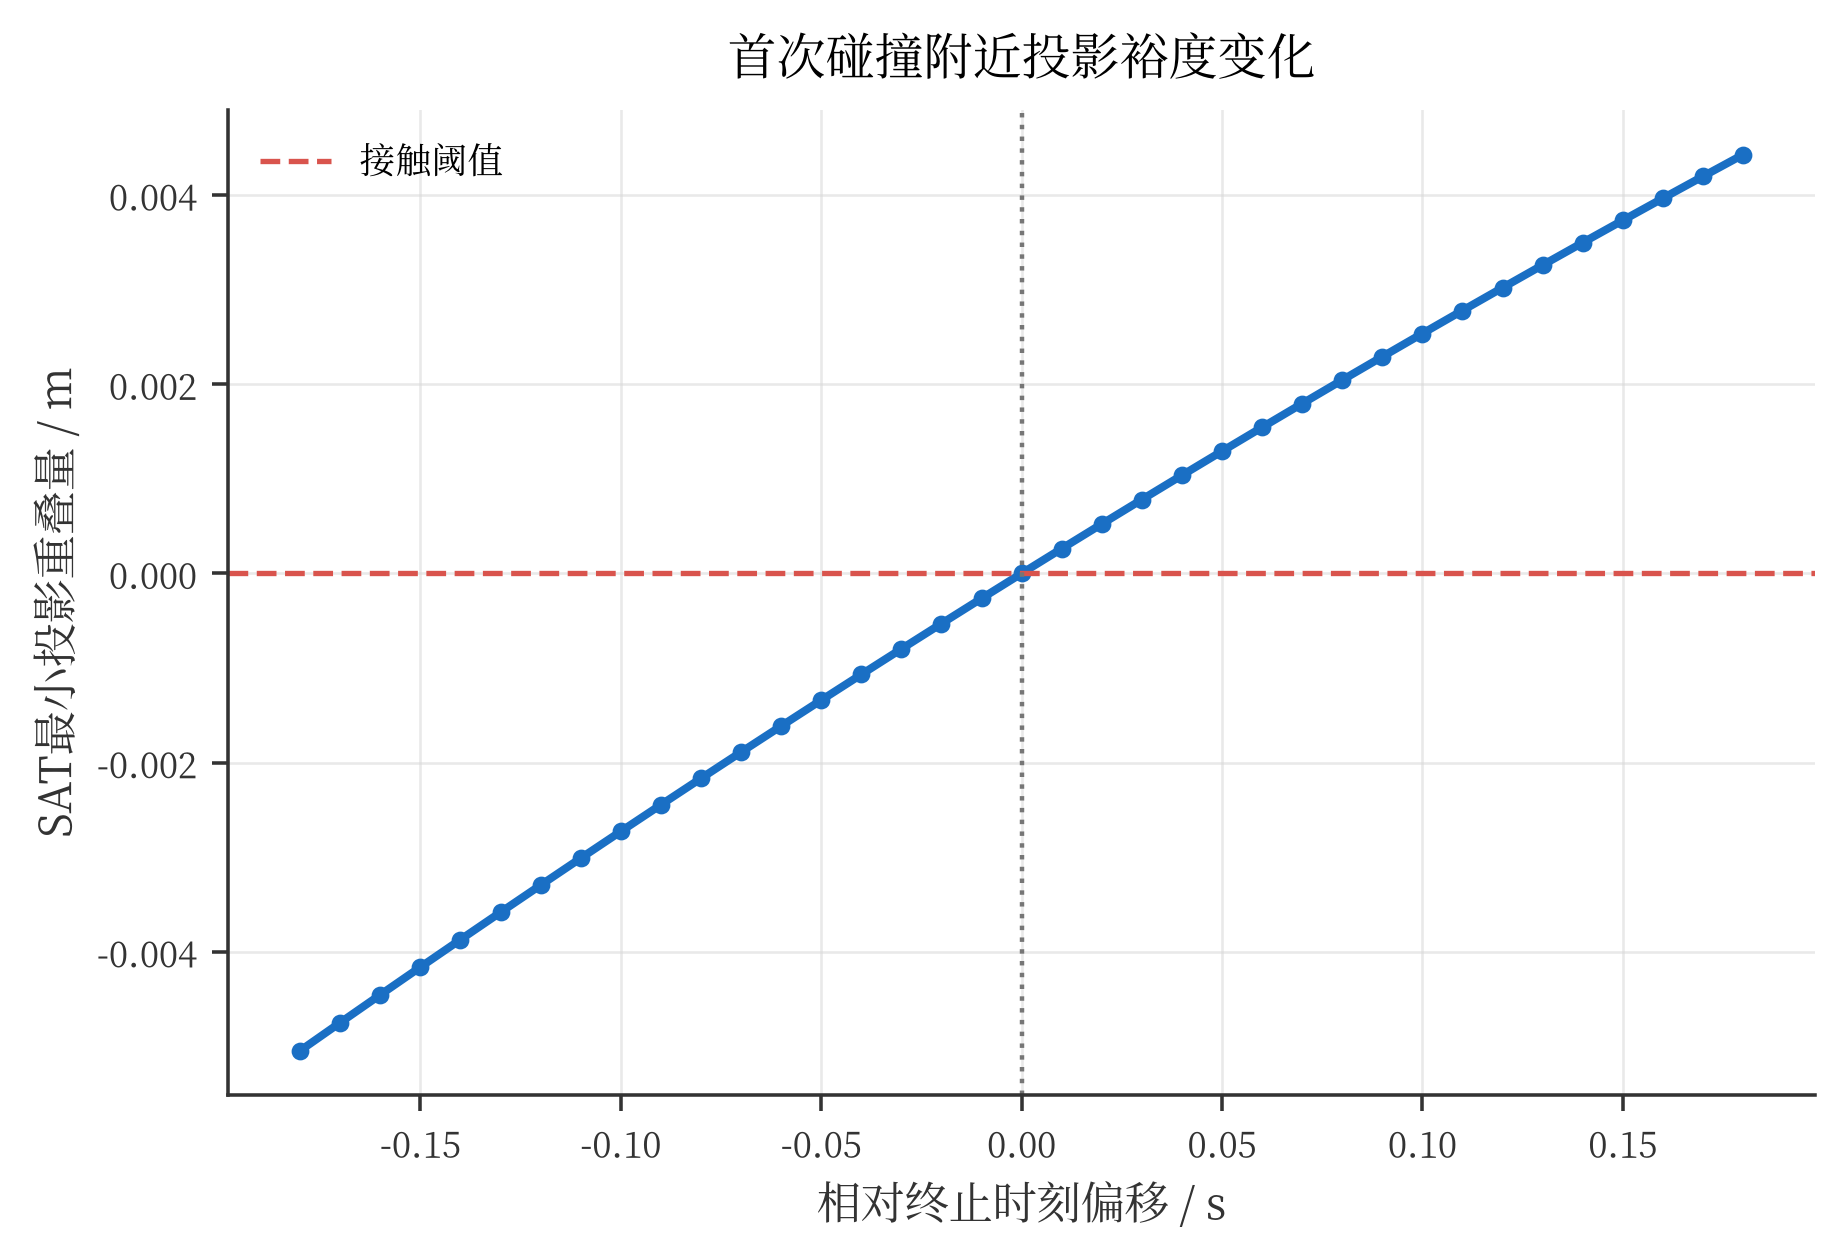
\includegraphics[width=0.88\textwidth]{figures/python/q2_collision_margin_trace.png}
\caption{首次碰撞附近最小投影裕度变化}
\label{fig:q2-collision-margin-trace}
\end{figure}

首次碰撞附近板凳龙的整体位置示意图如下，用于标明龙头与第8节板凳的相对位置关系。

\begin{figure}[H]
\centering
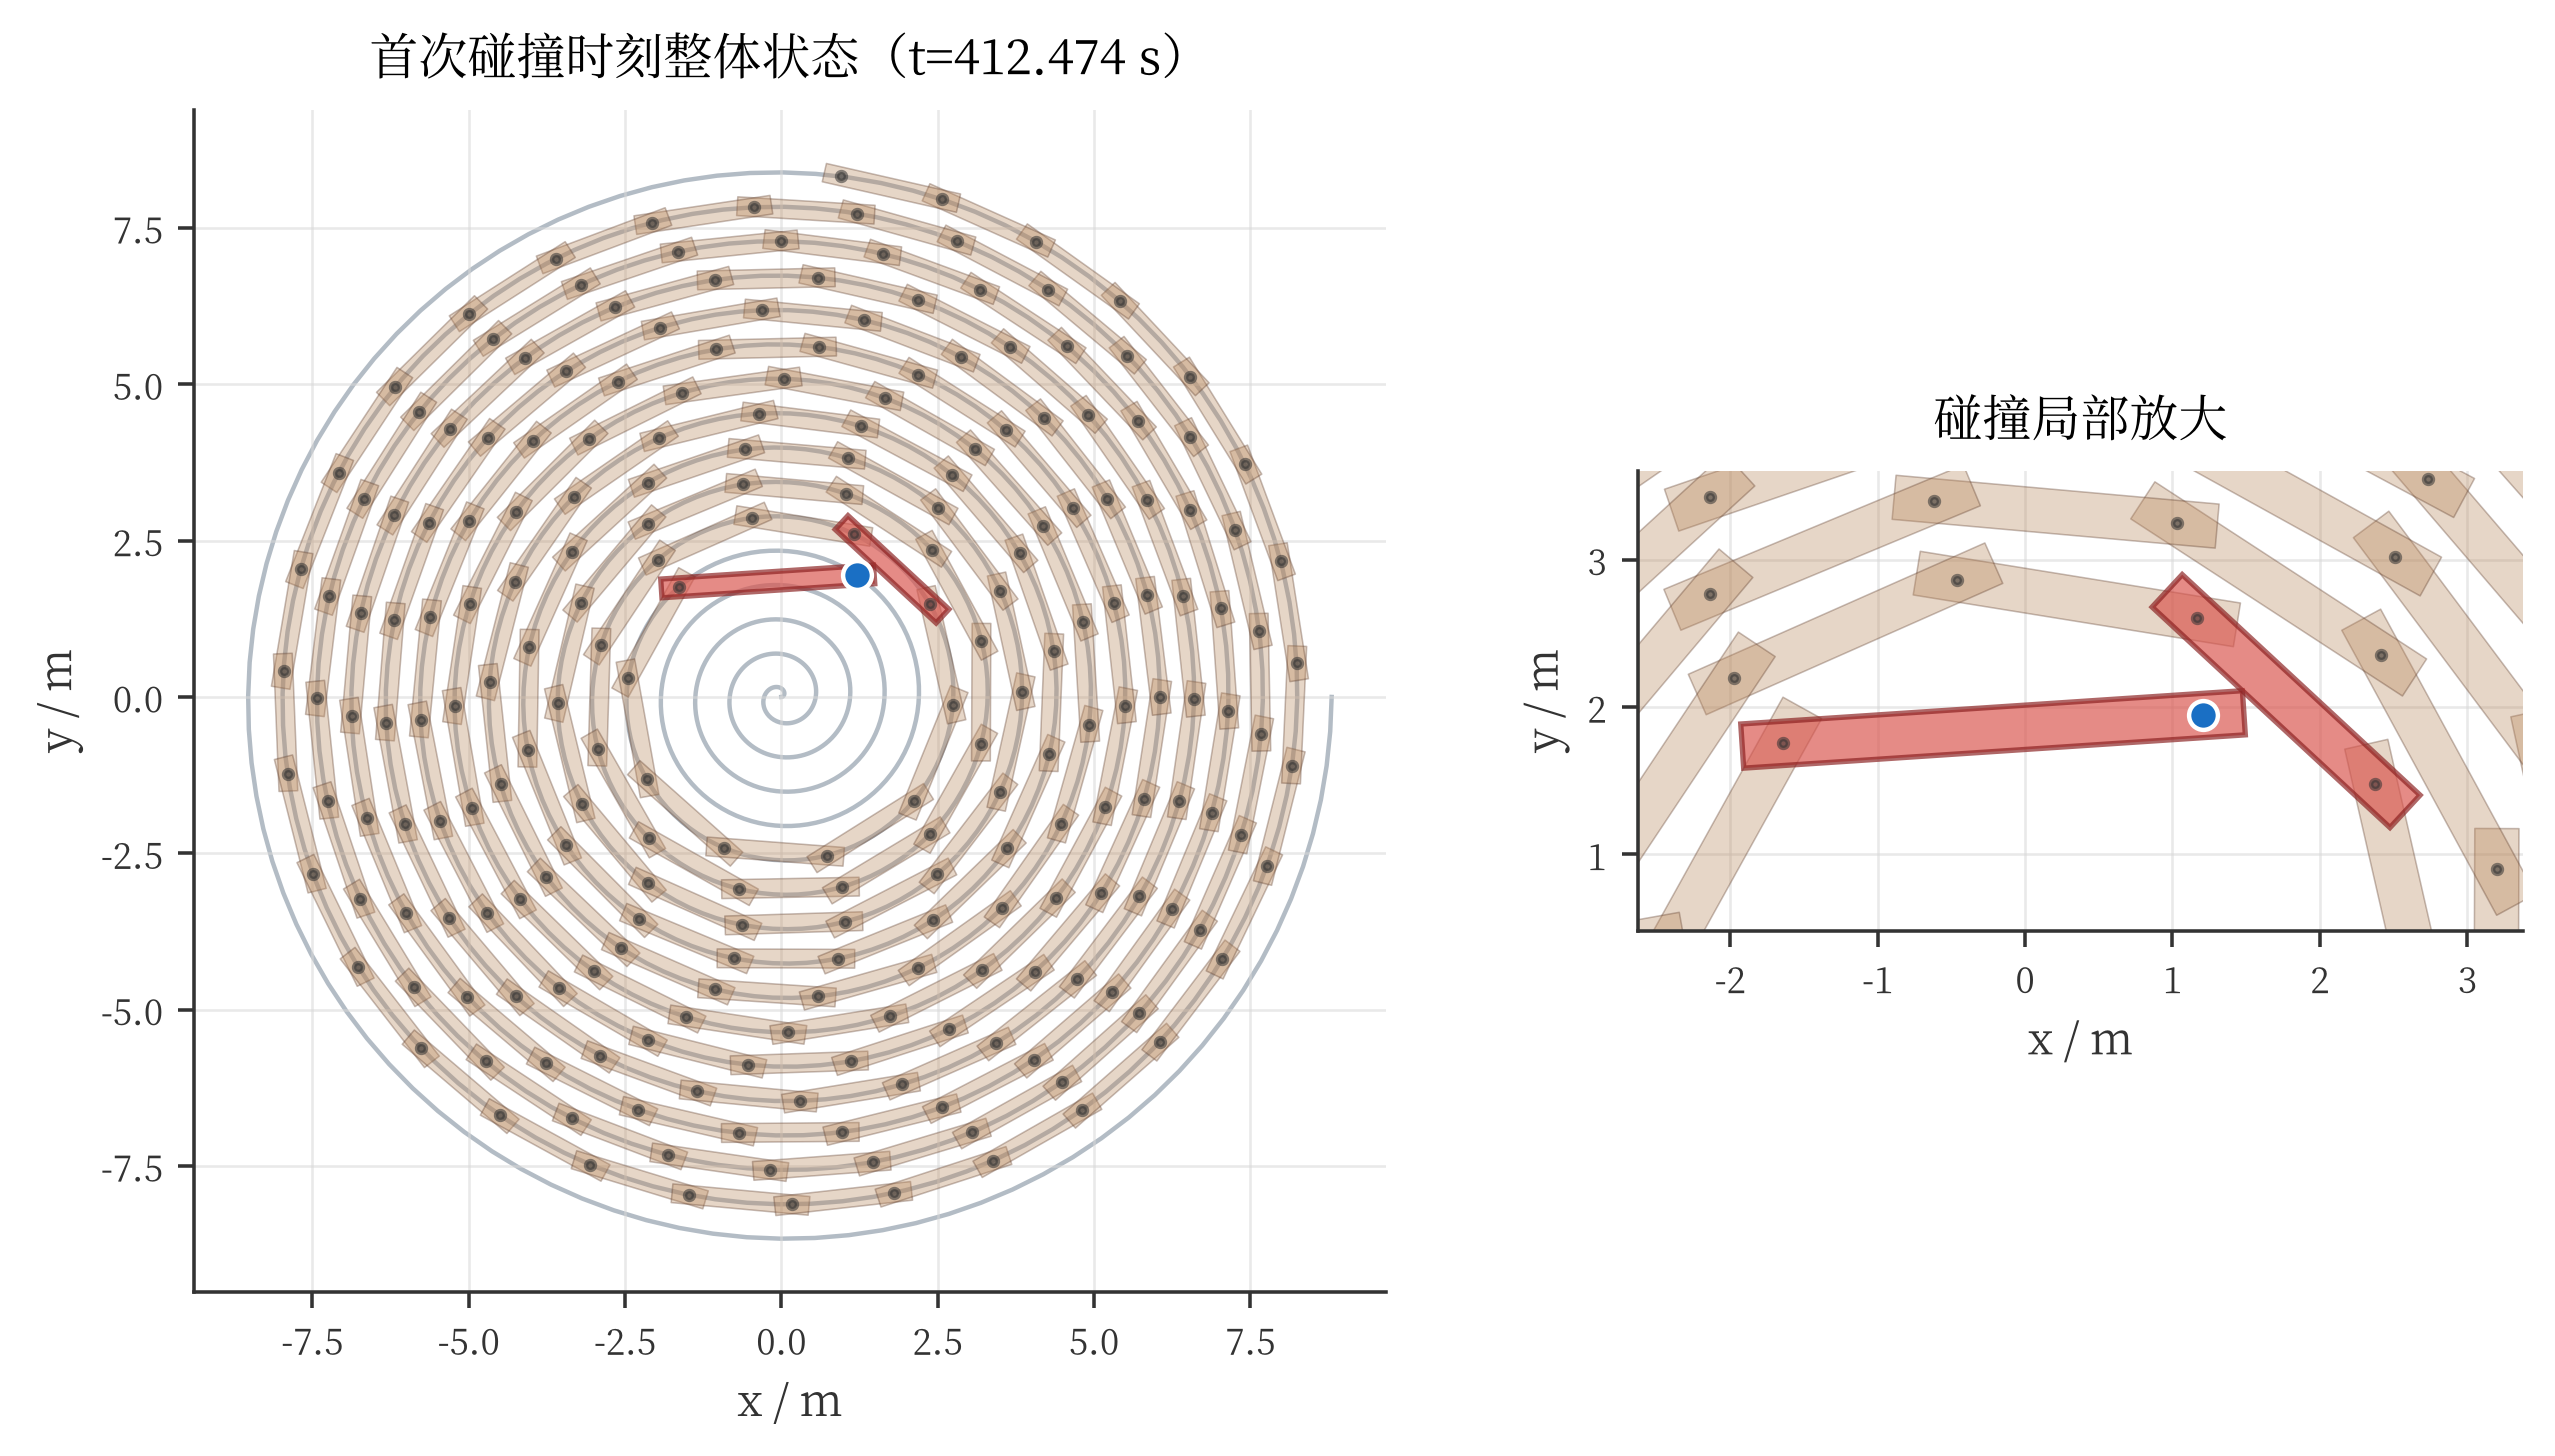
\includegraphics[width=0.92\textwidth]{figures/python/q2_collision_snapshot.png}
\caption{首次碰撞时刻附近板凳龙位置示意}
\label{fig:q2-collision-snapshot}
\end{figure}

终止状态已按附件二格式写入工作簿。该时刻全体把手速度范围为$0.973$到$1.000$ m/s。

\begin{table}[H]
\centering
\caption{问题二终止状态抽样表}
\label{tab:q2-terminal}
\begin{tabularx}{\textwidth}{lCCC}
\toprule
项目 & $x$ (m) & $y$ (m) & 速度 (m/s)\\
\midrule
龙头 & 1.209931 & 1.942784 & 1.000000\\
第1节龙身 & -1.643792 & 1.753399 & 0.991551\\
第51节龙身 & 1.281201 & 4.326588 & 0.976858\\
第101节龙身 & -0.536246 & -5.880138 & 0.974550\\
第151节龙身 & 0.968840 & -6.957479 & 0.973608\\
第201节龙身 & -7.893161 & -1.230764 & 0.973096\\
龙尾（后） & 0.956217 & 8.322736 & 0.972938\\
\bottomrule
\end{tabularx}
\end{table}

\subsection{小结}
问题二的终止时刻求解可以概括为“定义碰撞判定函数$\chi(t)$，定位其由0跃迁到1的临界点”。分离轴原理提供了矩形相交判定的数学基础，扫描与二分则提供了临界时刻的数值定位方式。该处理方式比仅凭中心线或经验距离判断更符合题目的实体碰撞要求。
